% Qastrocam-g2
% Copyright (C) 2009   Blaise-Florentin Collin

% This program is free software; you can redistribute it and/or
% modify it under the terms of the GNU General Public License v2
% as published by the Free Software Foundation.

% This program is distributed in the hope that it will be useful,
% but WITHOUT ANY WARRANTY; without even the implied warranty of
% MERCHANTABILITY or FITNESS FOR A PARTICULAR PURPOSE.  See the
% GNU General Public License for more details.

% You should have received a copy of the GNU General Public License
% along with this program; if not, write to the Free Software
% Foundation, Inc., 51 Franklin Street, Fifth Floor, Boston,
% MA  02110-1301, USA.

\documentclass[11pt,a4paper]{book}
%=============== En−Tete ===============
\usepackage[french]{babel}
\usepackage{a4wide}
%\usepackage[T1]{fontenc}
%\usepackage[cyr]{aeguill}
%\usepackage{epsfig}
%\usepackage{amsmath, amsthm}
\usepackage{amsfonts,amssymb}
%\usepackage{SIunits}
\usepackage{graphicx}
\usepackage{float}
\usepackage{url}
\bibliographystyle{plain}

\DeclareGraphicsExtensions{.png}

\pdfcompresslevel9

\title{Manuel d'utilisation Qastrocam-g2 vers. 5.0}
\author{Thx8411 \url{thx8411@users.sourceforge.net}}
%=============== Corps ===============
\begin{document}

\maketitle

\tableofcontents

\chapter{Pr\'esentation}

\paragraph*{}
Qastrocam-g2 est un logiciel dont le but est de permettre la capture d'images
astronomiques sous Linux. Il s'agit d'une variante du logiciel Qastrocam d\'evelopp\'e
par F. Sicard et modif\'e par moi-m\^eme pour mes propres besoins. Qastrocam-g2 \'etant
assez cibl\'e sur mon propre mat\'eriel, je vous recommande d'utiliser le Qastrocam
original si vous rencontrez quelques soucis, celui-ci pr\'esentant sans doute une
meilleure stabilit\'e. Bien que travaillant sur deux variantes du m\^eme logiciel, F.
Sicard et moi-m\^eme \'echangeont afin d'enrichir le logiciel original.

\paragraph*{}
Qastrocam et Qastrocam-g2 sont h\'eberg\'es sur SourceForge aux adresses suivantes :

\paragraph*{}
\begin{itemize}
\item \url{http://sourceforge.net/projects/qastrocam/}
\item \url{http://sourceforge.net/projects/qastrocam-g2/}
\end{itemize}

\paragraph*{}
Qastrocam-g2 est sous licence GPL version 2.

\paragraph*{Historique}
\paragraph*{}
\renewcommand\labelitemi{\textbullet}
\begin{itemize}
\paragraph*{}
\item vers. 4.9
\begin{itemize}
\item basic lucam-recorder SER format support
\item QHY5 short exposures enabled
\item Frame scaling mode is now stored
\item The telescope speed is now stored
\item QHY5 previous exposure time value stored
\item QHY5 exposure time better slider
\item QHY5 previous gain value stored
\item QHY5 available frame sizes changed
\item Gamma bug on philips cameras fixed
\item No more time limites for QHY5 telescope moves
\item Nexstar protocol support added (1.6+)
\item The camera display can now be resized/scrolled
\item QHY5 gain value fixed
\paragraph*{}
\end{itemize}
\item vers. 4.8
\begin{itemize}
\item avifile-win32-plugin package bug on amd64 fixed
\item fifo self created if needed
\item dark frames generation added (average and median methods)
\item To many available frame sizes bug fixed
\item Autoguiding slew speed can now be changed on some devices
\item Registax compatible avi output added
\item QHY5 guiding port supported
\item Telescope configuration bug fixed
\item LX200 protocole supported via autostar
\item QHY5 imager support added
\item software bilinear scaling added
\item night vision mode added
\item bias pre-processing added
\item added bayer color separation
\item better sources portability
\item pdf manual building is now optional
\item a bit of SDL speed up
\item mmap buffer number change
\item V4L2 objects re-organised
\item DC60 extras controls added
\item long exposure mode support added for astroeasycap
\item better scmod handling
\item gui palette bug fixed
\item spca505 palette support added
\item jpeg palette resize bug fixed
\item B/W frames optimisation (speed x2)
\item uyvy palette support added
\item gui re-draw to avoid space loose
\item flat pre-processing added
\item dark pre-processing added
\item pre-process tab added
\item de-bayer moved to pre-process
\item the old conf file isn't compatible with this new version anymore
\item mirror module option removed
\end{itemize}
\paragraph*{}
\item vers. 4.7
\begin{itemize}
\item release number added in main window caption
\item better colors in binning mode
\item yuv420 to yuv444 bug fixed
\item V4L generic forcing option removed
\item basic v4l(1) support is back
\item vesta framerate/size change bug fixed
\item demosaic optimisation (speed x2)
\item jpeg palette support added
\item better frame size detection
\item much better lx frame detection
\item settings can be changed in gui
\item better color conversions
\item some options removed/changed (can be accessed by gui)
\item cout is redirected to a log file
\item avi lossless recording added (huffyuv)
\item option '-i' not available anymore (now useless)
\item device source can now be changed in gui
\item support added for BA81 palette
\item option '-p' not available anymore (now useless)
\item chosen palette now saved in the settings file
\item palette and mode now saved for each diffrent device
\item source combobox added
\item palette combobox added
\item debian packaging changed for multi-platform
\end{itemize}
\paragraph*{}
\item vers. 4.6
\begin{itemize}
\item now saving avi in raw rgb24 or 8 bits grey depending on frame type
\item many memory bugs/leaks fixed
\item FITS-GZ output removed
\item ccvt no more used     
\item webcam RGB palette now fully supported
\item native format is yuv444 instead yuv420 for better colors
\item minor GUI modifications
\item all file formats now support raw color frames
\item supports binning
\item snapshot button disabled when using AVI
\item supports software cropping
\item frame size now only limited by INT\_MAX
\item supports frame scaling (default) and hardware cropping (centered)
\end{itemize}
\paragraph*{}
\item vers. 4.5
\begin{itemize}
\item fixed a palette detection bug
\item partialy detects control options
\item everything migrated to v4l2
\item empty capture file name issue fixed
\item capture file name size no more limited
\item optimisation flags now applies on all the code
\item use "select" to notifie new frames with V4L2 devices
\item settings file name can now be forced
\item usage of V4L generic can now be forced
\item frame size limit becomes 8192x8192 (should be enough..)
\item v4l1 no more supported
\item yuv420i no more supported
\item Icons moved and changed to avoid conflicts with the qastrocam package
\item v4l generic lx frame selection now use max instead of mean pixel value
\end{itemize}
\paragraph*{}
\item vers. 4.4
\begin{itemize}
\item Removed useless image format (keeping FITS, FITS-GZ, AVI, BMP, PNG)
\item Removed obsolete parport LX control
\item Levels (inverted/normal) can be set for APM telescope
\item Levels (inverted/normal) can be set for // port LX
\item APM telescope and // port LX may now share the same port with ppdev and lp devices
\item V4L generic palette can be forced using -p option
\item Supports ppdev and standard lp ports with the "latch mod" (for "usb to //" devices)
\item Small yuyv to yuv420p speed improvement
\item Documentation about the "latch" // mod added
\item Active V4L input and palette displayed in gui
\item User manual added (french only at this time, sorry)
\item LX mode for V4L generic added (serial and //)
\item Binary compiled with -O3 (forgot in previous versions)
\item Binary target is now i686
\item autoconf warning fixed
\item Minor cosmetic fix
\item RGB24 palette support (luminance only)
\item V4L generic "hot" resize supported for all devices
\end{itemize}
\paragraph*{}
\item vers. 4.3
\begin{itemize}
\item YUYV palette support
\item Gnome menu entry and icon included in the debian package
\item V4L generic devices source can now be choosen. Choice is stored for each device
\item ccvt updated to 0.3 (no more asm)
\item File format, raw mode, resolution, level inversion, telescope device and lx device 
 are now stored and restored
\item Now supports level inversion on serial and led SCmod via command line
\item Enhanced V4L generic frame size support
\item Bugs fixed
\end{itemize}
\paragraph*{}
\item vers. 4.2rc2
\begin{itemize}
\item Version numbering changed vers. 4.2.2rc2 becomes 4.2rc2
\end{itemize}
\paragraph*{}
\item vers. 4.2.2rc2
\begin{itemize}
\item Quit button now quit on release
\item Bugs fixed
\end{itemize}
\paragraph*{}
\item vers. 4.2.2rc1
\begin{itemize}
\item Many bugs fixed
\item Sources cleaned
\end{itemize}
\paragraph*{}
\item vers. 4.2.2 beta BFC Fork
\begin{itemize}
\item You may generate tracking files, compatible with iris files, with "-t file -dt <filename>"
  Can be used with PEAS
\item Project renamed to qastrocam-g2
\end{itemize}
\paragraph*{}
\item vers. 4.2.1 beta BFC Fork
\begin{itemize}
\item The SCmod serial device can now be choosen with the -dx option
\item Some spelling error fixed
\end{itemize}
\paragraph*{}
\item vers. 4.2.0 beta BFC Fork
\begin{itemize}
\item Added serial SC mod support using F. Sicard previous work (roots version, to be "cleaned")
\item Type mismatch correction in LED SCmod
\item Some spelling errors fixed
\end{itemize}
\paragraph*{}  
\item vers. 4.1.0 pre 17082009 : original qastrocam sources used
\end{itemize}

\chapter{Capture}

\section{Mat\'eriel support\'e}

\paragraph*{}
Qastrocam-g2 supporte deux types de p\'eriph\'eriques de capture, les p\'eriph\'eriques V4L1 
g\'en\'eriques ainsi que les sp\'ecificit\'es de certains pilotes (notamment pour les webcams
CCD philips). Le passage aux pilotes V4L2 est pr\'evu pour la version 4.5.

\subsection{P\'eriph\'eriques V4L g\'en\'eriques}

\paragraph*{}
Le support des p\'eriph\'eriques g\'en\'eriques V4L est encore en plein d\'eveloppement. Un
bon nombre d'informations sur le support ou non de vos p\'eriph\'eriques est affich\'e dans
la console lors du lancement de qastrocam-g2 en ligne de commande. Le p\'eriph\'erique doit
 \^etre  connect\'e avant le lancement du logiciel. Ces informations seront, \`a terme, 
 accessibles par l'interface graphique.

\paragraph*{} 
En cas de soucis, un  appel \`a la commande
 {\tt dmesg} juste apr\`es le branchement peut vous aider \`a identifier le probl\`eme. 

\subsubsection{Modes d'acc\`es}

\paragraph*{}
Qastrocam-g2 g\`ere deux des trois m\'ethodes d'acc\`es propos\'ees par les API V4L : la m\'ethode
{\tt read/write} et la m\'ethode {\tt mmap}, ce qui couvre la quasi totalit\'e des pilotes V4L
disponibles. La m\'ethode {\tt mmap} permet des acc\`es directes \`a la m\'emoire du pilote,
assurant ainsi des temps d'acc\`es plus faibles. Cette m\'ethode est donc utilis\'ee par d\'efaut.
En cas de probl\`eme, qastrocam-g2 bascule automatiquement sur la m\'ethode {\tt read/write}. Ceci
peut occasionner un l\'eger d\'ecalage entre l'image captur\'ee et l'image vue. 

\subsubsection{Sources vid\'eo}

\paragraph*{}
Lorsque le p\'eriph\'erique propose plusieures sources de captures vid\'eo (Tuner, Composite et
S-VHS, par exemple), qastrocam-g2 utilise la source par d\'efaut. Il est cependant possible de
choisir cette source via l'option {\tt -i}. La liste des sources disponibles est affich\'ee dans
la console lors du lancement.

\paragraph*{}
L'option choisie, si elle est valide, est alors enregist\'ee dans le fichier de configuration.

\subsubsection{R\'esolutions}

\paragraph*{}
La r\'esolution maximale est pour l'instant la r\'esolution du standard PAL, soit 720x576 pixels.
La majorit\'e des mat\'eriels de capture vid\'eo permettent le choix d'une r\'esolution quelconque
entre les r\'esolutions minimales et maximales (pourvu que celles-ci soient multiples de quatre ou
de huit). Le choix entre toutes ces r\'esolutions possibles est rarement pertinent. Qastrocam-g2
propose donc les r\'esolutions disponibles du maximum au minimum, chaque r\'esolution \'etant
le quart (en nombre de pixels) de la pr\'ec\'edente.

\paragraph*{}
Ainsi, les r\'esolutions disponibles seront souvent les suivantes en PAL :

\paragraph*{}
\begin{itemize}
\item 720x576
\item 360x288
\item 180x144
\end{itemize}

\paragraph*{}
Elles seront souvent les suivantes en NTSC :

\paragraph*{}
\begin{itemize}
\item 640x480
\item 320x240
\item 160x120
\end{itemize}

\subsubsection{Palettes}

Qastrocam-g2 supporte les palettes V4L suivantes. Ces palettes sont test\'ees par ordre de qualit\'e,
comme pr\'esent\'ees dans cette liste :

\paragraph*{}
\begin{itemize}
\item RGB24 (support partiel, luminance uniquement)
\item YUYV (YUV422)
\item YUV420p (Planar)
\item 8 bits grey
\end{itemize}

\paragraph*{}
Le support de la palette JPEG est pr\'evu pour les versions futures. Bien que la qualit\'e
de cette palette soit souvent m\'ediocre, elle permettra l'utilisation de nombreuse petites
webcams du commerce pour l'autoguidage.

\subsubsection{Contr\^oles}

\paragraph*{}
Les contr\^oles disponibles (luminosit\'e, contraste, etc.) sont ceux propos\'es par le pilote
V4L. Ils sont accessibles dans l'interface graphique par l'interm\'ediaire de curseurs.

\subsubsection{Nombre d'images par secondes}

\paragraph*{}
Le nombre d'images par seconde (framerate) utili\'e est celui du standard vid\'eo d\'etect\'e,
soit 25 images par secondes pour le PAL et 30 images par secondes pour le NTSC. Ceci peut \^etre
modifi\'e par l'utilisation du module de pose longue.  

\subsection{Webcams "VESTA"}

\subsection{Webcams "OV511"}

\chapter{Mode "poses longues"}

\section{Interfaces support\'ees}

\subsection{Port s\'erie}

\subsection{Port parall\`ele}

\subsection{Toucam LED}

\section{V4L g\'en\'erique}

\section{Cameras PHILIPS}

\chapter{Enregistrement}

\section{Formats}

\section{Snapshot}

\section{S\'equence}

\section{Propri\'et\'es}

\chapter{Autoguidage}

\section{Interface graphique}

\section{Interfaces T\'el\'escopes}

\subsection{APM}

\subsection{AutoStar}

\subsection{Fifo}

\subsection{Mcu}

\subsection{Mts}

\subsection{File}

\chapter{Accumulation}

\chapter{Alignement}

\chapter{Options de ligne de commande}

\chapter{Le fichier de configuration}

\appendix

\chapter{Compilation de Qastrocam-g2}

\section{Packages n\'ec\'essaires}

\begin{itemize}
\item autoconf
\item g++
\item libqt3-mt-dev
\item libavifile-0.7-dev
\item libcfitsio3-dev
\item libsdl1.2-dev
\item libdts-dev
\item libusb-dev
\item libqwtplot3d-qt3-dev
\end{itemize}

\section{Configuration de la plate-forme}

\section{Compilation et instalation}

\section{G\'en\'eration d'un package debian}

\chapter{Modification "latch"}

\section{Introduction}

\paragraph*{}
Longtemps, le port parall\`ele a constitu\'e un outil de choix pour
interfacer un ordinateur personnel au monde ext\'erieur, notamment en
astronomie amateur. Cependant, depuis quelques ann\'ees, ces ports
disparaissent de nos machines, et surtout des machines portables,
pourtant tr\`es utiles \`a l'astronome nomade.

\paragraph*{}
Le port souverain est aujourd'hui l'USB, mais ce port ne permet pas l'acc\`es
 direct \`a des niveaux \'electriques TTL. Les solutions envisageables
permettant le contr\^ole direct de ces niveaux TTL bit \`a bit sont donc de
passer par un adaptateur. Il existe des interfaces USB/parall\`ele totalement
contr\^olables pour des applications industrielles ou d'instrumentation de 
laboratoire, mais \`a des prix non n\'egligeables. Pour disposer d'une 
interface \`a un prix raisonnable, il ne reste donc que les interfaces USB/s\'erie 
ou USB/parall\`ele standards du march\'e chinois, pour quelques dollars ou euro.

\paragraph*{}
Les adaptateurs USB/s\'erie on l'avantage d'\^etre totalement contr\^olables (sur les bits
de signalisation, du moins), mais ils ne fournissent que deux bits en sortie et deux bits en
entr\'ee. C'est la solution utilis\'ee par la modification longue pose s\'erie (utilisant
les lignes {\tt DTR} et {\tt RTS}). Il faut cependant adapter les niveaux de tension 
(diverses solutions existent, avec des jeux de r\'esistances, des transistors, des diodes
 zener, etc), les liaisons RS232
 fonctionnant en +/-12V. Malheureusement, cette solution ne fournie pas suffisamment de 
 sorties pour contr\^oler \`a la fois une camera longue pose et l'autoguidage d'une
 monture. Pour cela, point d'autre salut que le port parall\`ele.

\paragraph*{} 
La vie \'etant sans doute trop simple, il n'est bien s\^ur pas possible de piloter directement
les niveaux de sortie d'un adaptateurs USB/parall\`ele. En effet, ces adaptateurs ne simulent pas
un port "parall\`ele", mais un port "imprimante". Cela signifie que le contr\^ole du p\'eriph\'erique
n'intervient qu'en couche haute, ou pour \^etre plus claire, qu'il est impossible de contr\^oler 
les bits de signalisation du ports, et que celui-ci n'accepte d'\'echanger des donn\'ees que
s'il est connect\'e \`a une imprimante, ou au moins quelque chose qui se comporte comme tel.

\paragraph*{}
C'est l\`a qu'intervient la modification "latch", qui consiste \`a ins\'erer le minimum 
d'\'electronique permettant de simuler le comportement d'une imprimante, afin de disposer tout
de m\^eme des huit bits de donn\'ees disponibles sur le port. J'appelle cette modification
"latch" car le plus gros de l'\'electronique est constitu\'e d'un composant TTL qui
verrouille les niveaux de sortie du port, un "latch" en anglais (un 74HC573 en l'occurrence qui 
peut \^etre remplac\'e par un 74HC574, voir un composant d'une autre s\'erie, type LS en fonction
 des disponibilit\'es), composant tr\`es courant \`a moins de un euro.

\paragraph*{}
Le plus gros du travail provient d'ici : \url{http://www.unixgarden.com/index.php/embarque/entreessorties-simples-sur-usb}, 
avec quelques petites modifications de confort. Une LED permet de voir si le montage est sous tension. Le 
montage est auto-aliment\'e. De plus, un "reset" de l'imprimante engendre un "reset" du
verrou. La porte inverseuse du 7404 est remplac\'ee par un petit inverseur \`a transistor, moins 
encombrant qu'un circuit int\'egr\'e complet.

\section{Explications}

\paragraph*{}
Nous avons connu les "yes cards", voici venir la "yes printer". Le principe de
 base de cette modification est de faire croire que les donn\'ees sont toujours lues
 correctement, que l'imprimante et toujours disponible, et que tout se passe toujours bien.
  Pour cela, une partie des
 signaux est directement renvoy\'ee \`a l'ordinateur, comme accus\'e r\'eception, et
 une autre for\c{c}\'ee au niveau bas. Le signal de 
 synchronisation sera utilis\'e pour stocker les donn\'ees dans le verrou.
 
 \paragraph*{}
 Un bon dessin \'etant bien mieux qu'un long discours, le sch\'ema est visible sur la figure~\ref{latch1}.
 
 \begin{figure}
 \center
 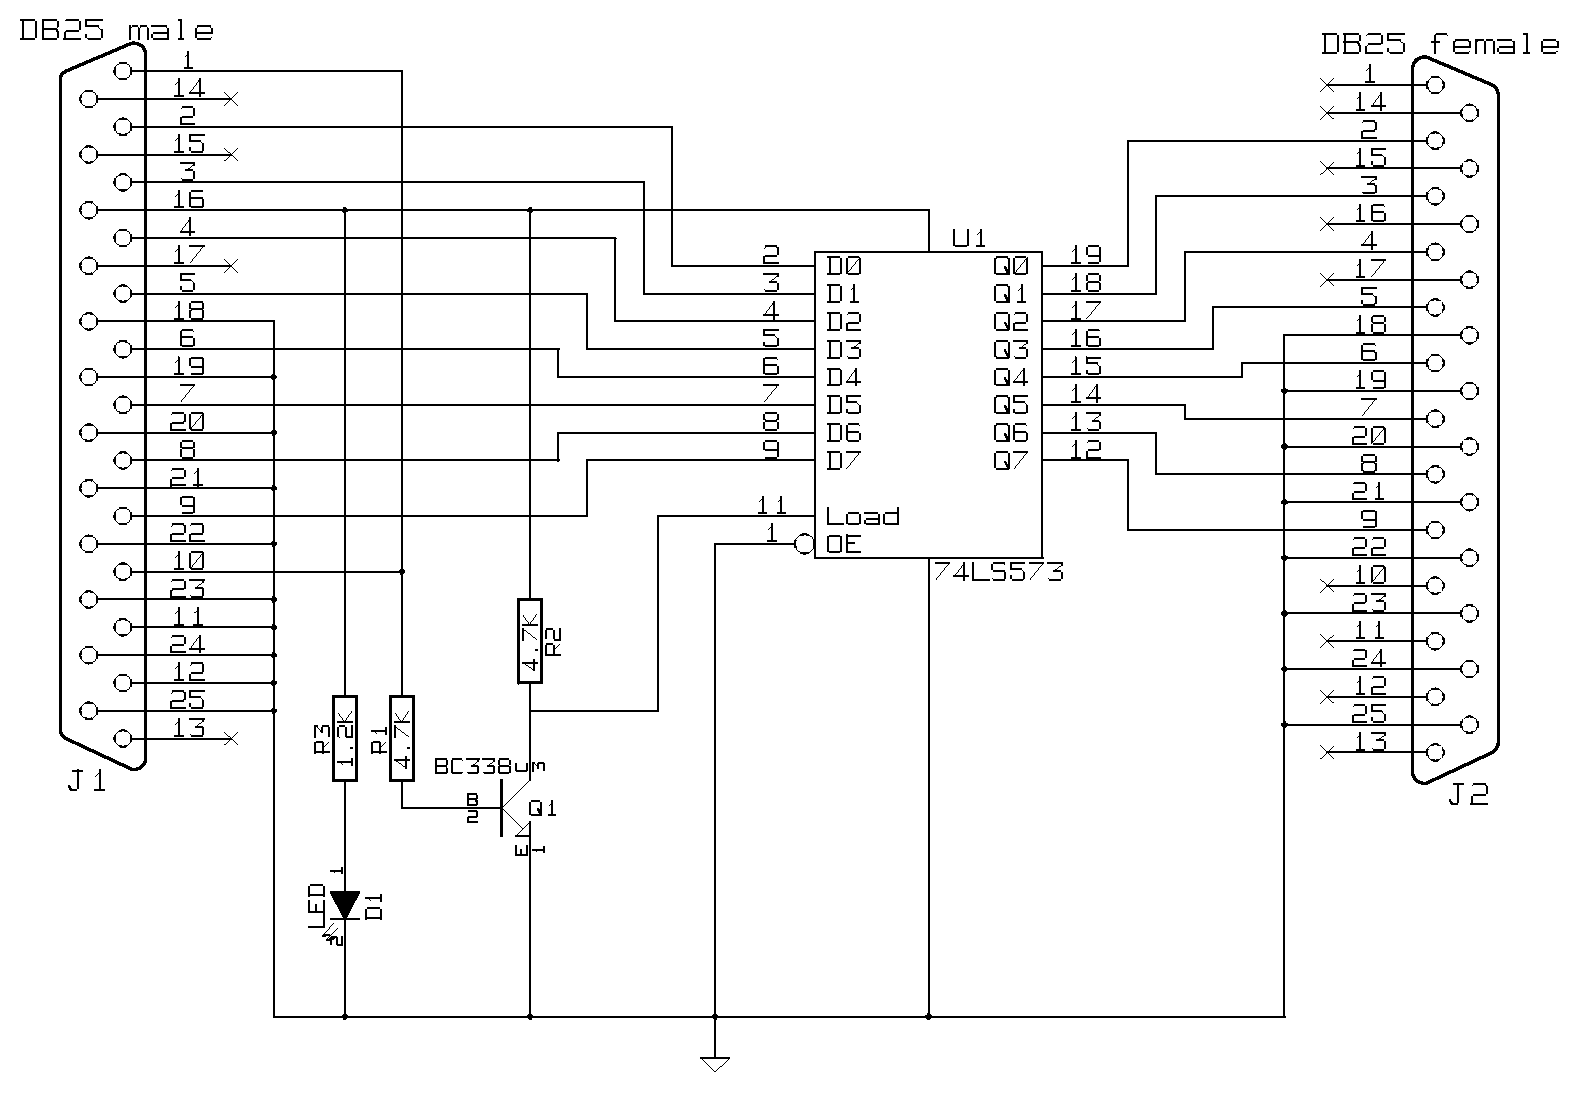
\includegraphics[scale=1.1]{./medias/latch1.png}
 \caption{sch\'ema}
 \label{latch1}
 \end{figure}
 
\paragraph*{}
Le PC se trouve cot\'e J1, et l'\'el\'ement ext\'erieur \`a contr\^oler cot\'e J2. Les pins \`a
la masse des deux connecteurs sont mises \`a la masse du montage, et les pins de donn\'ees 
respectivement connect\'ees \`a l'entr\'e et \`a la sortie du verrou. Sur J2, aucun des bits
de signalisation n'est report\'e. Normal, nous n'y avons de toute fa\c{c}on pas acc\`es.
C'est au niveau des bits de signalisation de J1 que les choses se jouent.

\paragraph*{}
Le signal {\tt INIT} (16) nous sert d'alimentation pour le montage. Il est en effet maintenu \`a
{\tt HIGH} par le PC, sauf lors de l'envoi d'un {\tt RESET} \`a l'imprimante, ce qui nous permet 
\'egalement de faire un {\tt RESET} du verrou. Ce signal alimente donc le verrou, un petit t\'emoin
\`a LED ainsi qu'un inverseur \`a transistor dont nous reparlerons plus loin. Il est \`a noter
que les signaux d'un port parall\`ele sont faits pour piloter des portes logiques, il est donc 
important d'en tirer le moins de courant possible. La LED sera donc de pr\'ef\'erence une LED
faible courant, avec une r\'esistance de limitation adapt\'ee. De toute mani\`ere, en application
astronomique, il est conseill\'e d'avoir le moins de lumi\`eres parasites possible, la LED et sa r\'esistance 
peuvent donc \^etre omises au besoin. De m\^eme pour les donn\'ees en sortie, il est imp\'eratif que 
celles-ci soient reli\'ees \`a des entr\'es haute imp\'edance.

\paragraph*{}
 Notre imprimante n'est jamais occup\'ee et a toujours du papier, les entr\'es {\tt BUSY} (11) et
 {\tt PAPEROUT} (12) sont donc reli\'ees \`a la masse. L'entr\'ee {\tt /ACK} (10) est directement reli\'ee
 \`a la sortie {\tt STROBE} (1). Notre imprimante accuse automatiquement r\'eception de tout ce
 qu'elle re\c{c}oit. {\tt STROBE}, via notre inverseur, pilote \'egalement le chargement de notre
 verrou. Sur notre verrou, les donn\'ees doivent \^etre en permanence disponibles en sortie,
 {\tt /OE} est donc mise \`a la masse.
 
 \paragraph*{}
 Les autres signaux, {\tt SELECT} (13), {\tt AUTOFEED} (14), {\tt ERROR} (15) et 
 {\tt SELECTIN} (17) n'ont pas besoin d'\^etre g\'er\'es, ils sont donc simplement ignor\'es. 
 
\section{Liste des composants}

\paragraph*{Base}
\begin{itemize}
\item J1 : connecteur DB25 pour circuit imprim\'e coud\'e m\^ale
\item J2 : connecteur DB25 pour circuit imprim\'e coud\'e femelle
\item R1, R2 : r\'esistances (entre 4.7K$\Omega$ et 10K$\Omega$)
\item Q1 : transistor NPN d'usage g\'en\'eral (ici un BC338)
\item U1 : 74573 ou 74574, s\'erie HC ou LS
\end{itemize} 

\paragraph*{Optionnels}
\begin{itemize}
\item R3 : r\'esistance (ici 1.2K$\Omega$, d\'epend de la LED)
\item D1 : LED 3mm basse consommation
\end{itemize}
 
\section{R\'ealisation}

\paragraph*{}
La r\'ealisation ne devrait pas poser de probl\`emes. Pour tous ceux qui n'ont pas les moyens
mat\'eriels de graver des circuits imprim\'es, le montage sur une plaque de test est assez
simple, vu le faible nombre de composants. Pour les autres, voici le typon (figure~\ref{latch2}) 
ainsi que la s\'erigraphie (figure~\ref{latch3}) du montage. Les pistes sont volontairement
tr\`es larges, en simple face, pour permettre une r\'ealisation facile avec les moyens du bord.

\paragraph*{}
Si tout se passe bien, vous devriez obtenir un circuit semblable \`a la figure~\ref{latch3}.

\begin{figure}
 \center
 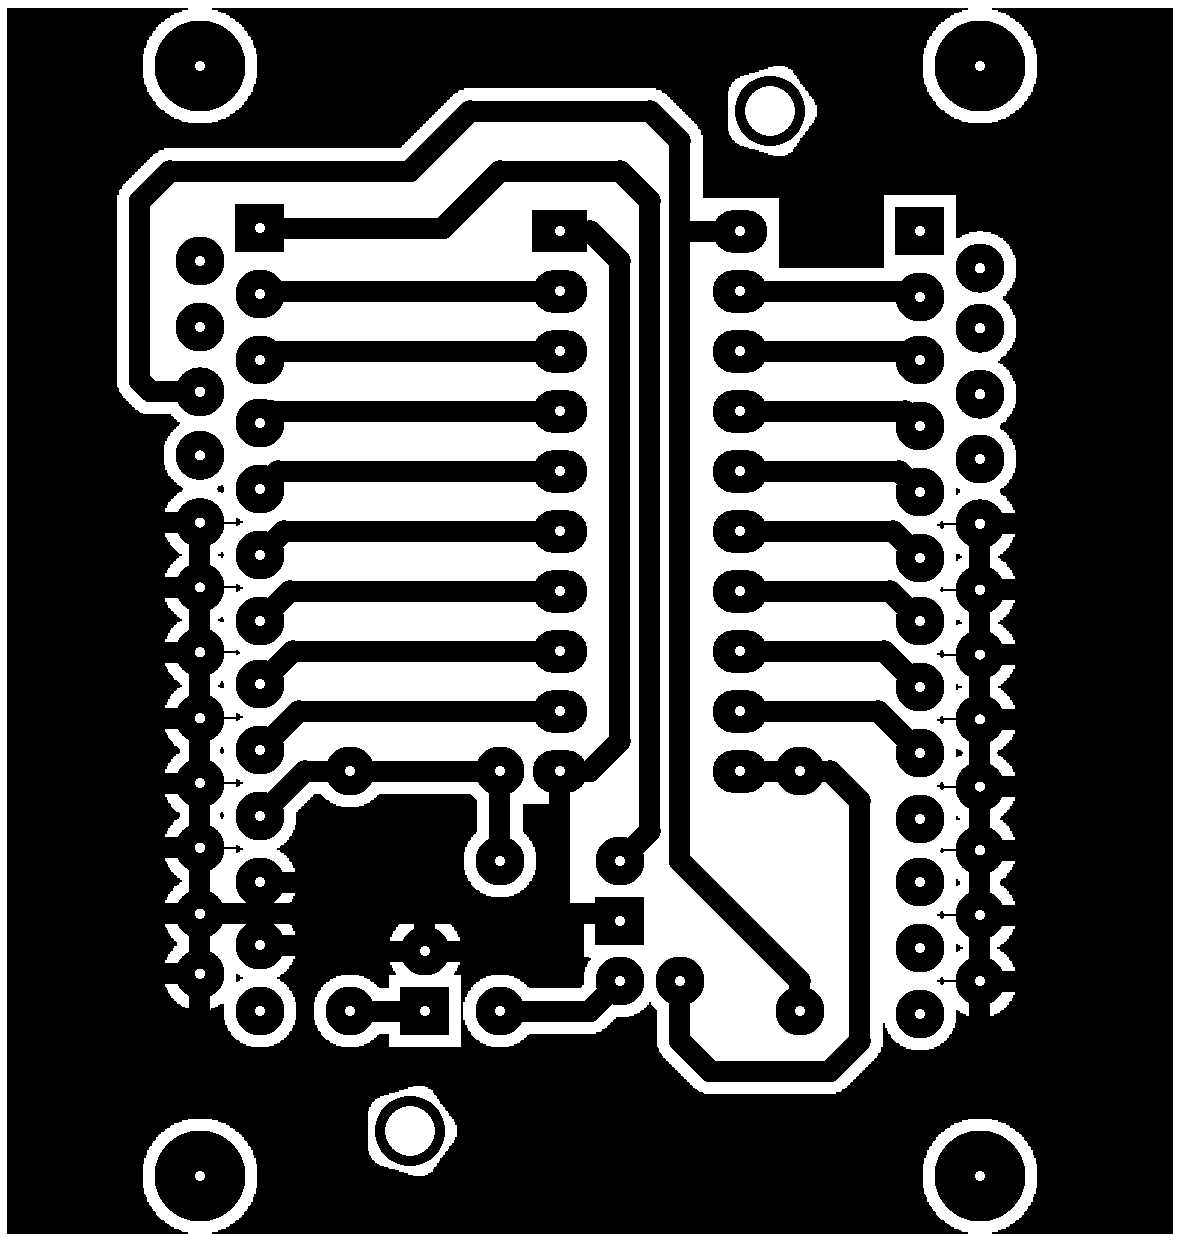
\includegraphics[width=5cm]{./medias/latch2.png}
 \caption{typon}
 \label{latch2}
 \end{figure}
 
 \begin{figure}
 \center
 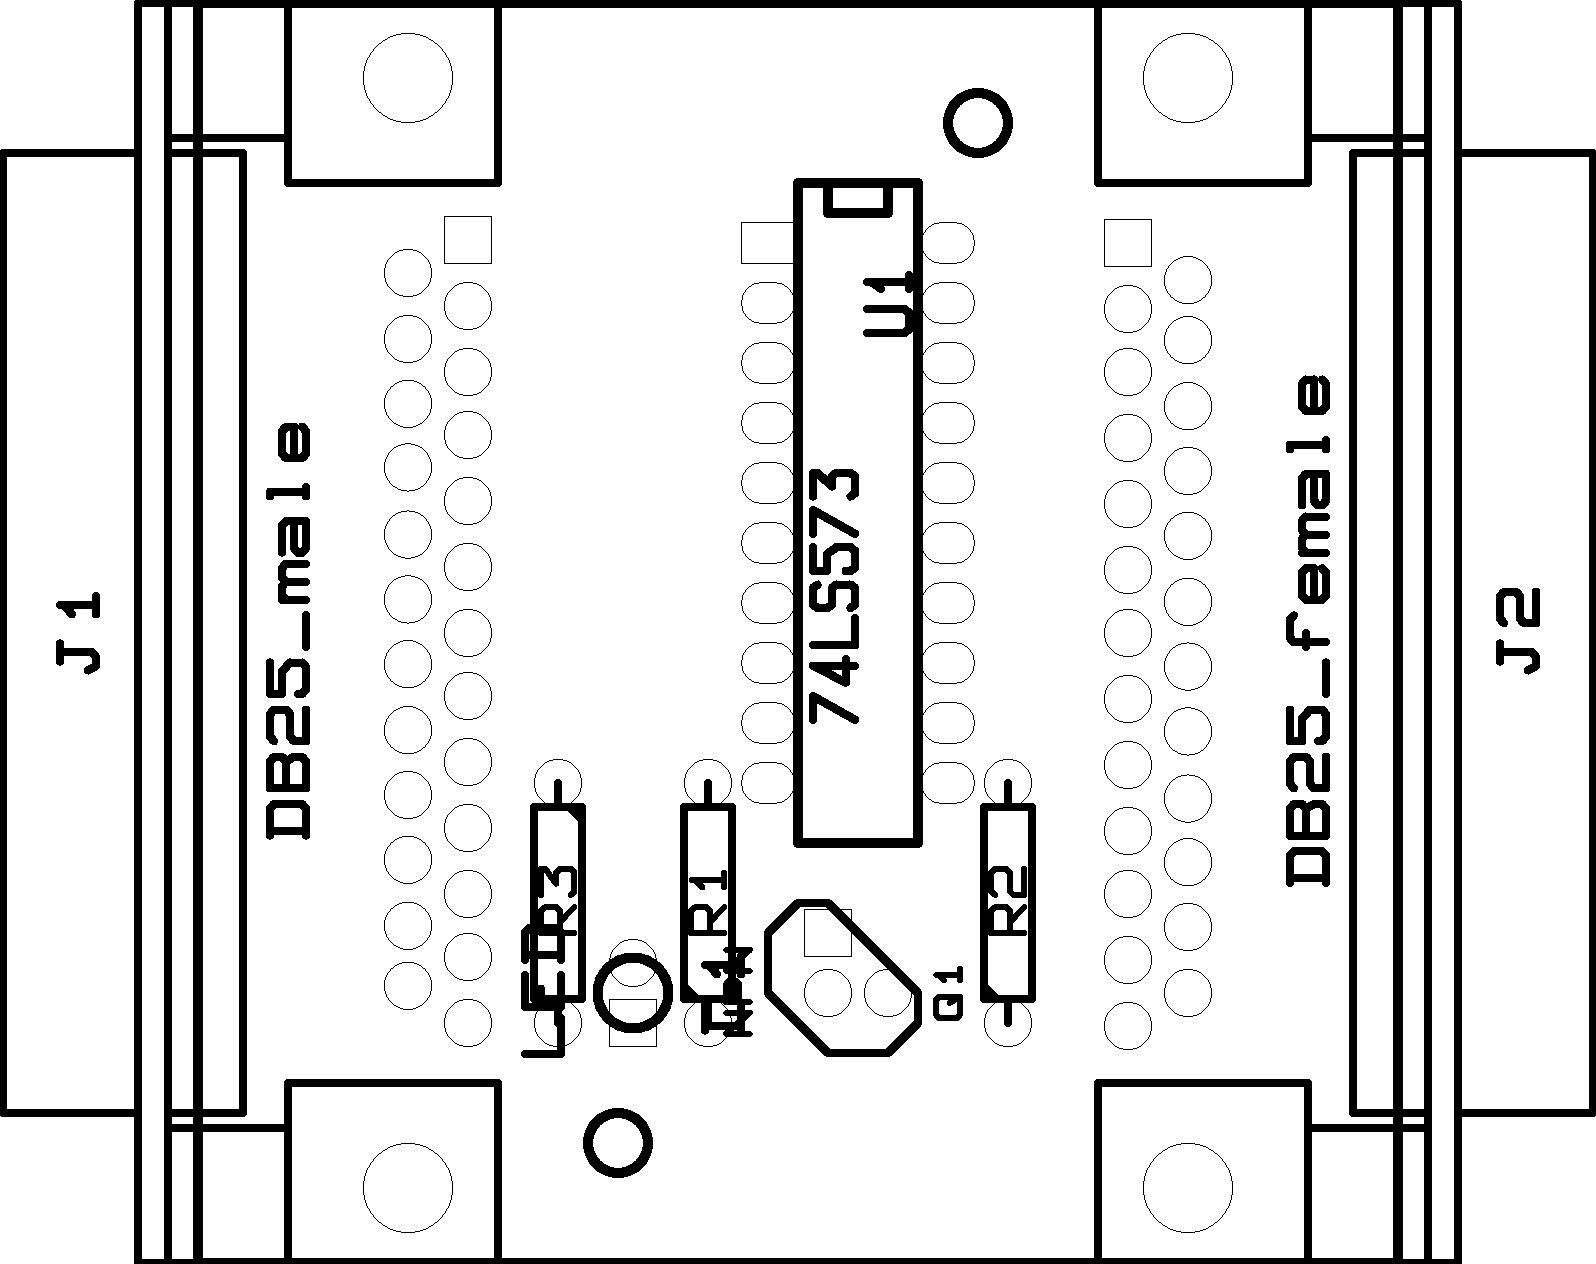
\includegraphics[height=52mm]{./medias/latch3.png}
 \caption{s\'erigraphie}
 \label{latch3}
 \end{figure}
 
 \begin{figure}
 \center
 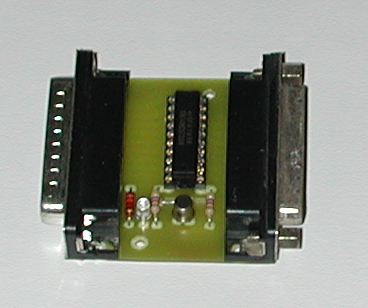
\includegraphics[scale=1.1]{./medias/latch4.png}
 \caption{montage}
 \label{latch4}
 \end{figure}
 
 \paragraph*{}
 Je vous recommande de placer tout ceci dans une petite boite, pour le prot\'eger de l'humidit\'e
 de vos sorties nocturnes...

\section{Mise en \oe uvre}

\paragraph*{}
Une fois ce petit montage branch\'e derri\`ere votre adaptateur USB/parall\`ele, il vous est
possible d'envoyer un octet directement en ouvrant le p\'eriph\'erique {\tt /dev/lp?} 
correspondant et en y \'ecrivant un {\tt unsigned char} (ou l\'equivalent dans un autre langage).
L'appel \`a la fonction {\tt ioctl} {\tt LPRESET} vous permet de r\'einitialiser le verrou. Je vous
recommande simplement d'ins\'erer un d\'elai d'une micro-seconde entre deux \'ecritures sur votre
port parall\`ele, vous respectez ainsi le "timing" standard de l'IEEE 1284.

\paragraph*{}
Je rappelle qu'il est tr\`es important de tirer le moins de courant possible de ce montage, et que
 l'\'equipement plac\'e en aval devra imp\'erativement disposer d'entr\'ees haute imp\'edance !

\listoffigures

\end{document}
